

\documentclass{beamer}
\usetheme{CambridgeUS}
\mode<presentation>
{
\setbeamercovered{transparent}
}
\usepackage{amsmath,amsfonts,amssymb}
\usepackage[center]{caption}
\usepackage[utf8]{inputenc}
\usepackage[ngerman]{babel}
\usepackage{graphicx}
\usepackage{svg}
\usepackage{pdfpages}
\usepackage{placeins}


% font definitions, try \usepackage{ae} instead of the following
% three lines if you don't like this look
\usepackage{mathptmx}
\usepackage[scaled=.90]{helvet}
\usepackage{courier}
\beamertemplatenavigationsymbolsempty 
\setbeamertemplate{footline}{}

%\usepackage[T1]{fontenc}
\title[Bachelorarbeit]{Untersuchung des Wachstums von Au auf Re(0001) mittels LEED und STM sowie
Aufbau und Test einer Sprühdepositionsapparatur}
\author[V. Grimm]{Verena Grimm}


\institute[]{
Vortrag zur Bachelorarbeit in Physik\\
Fachbereich Physik, Mathematik und Informatik (FB 08)\\
Johannes Gutenberg-Universität Mainz
}

\date{00.00.2014}


% Logo Universität
\titlegraphic{
\includegraphics[width=4cm]{bilder/JGU-Logo_sw_high.jpg}\hspace*{-8.5cm}}
% Logo auf jeder Seite rechts unten:
% \pgfdeclareimage[height=1.5cm]{university-logo}{bilder/JGU-Logo_sw_high.jpg}
%  \logo{\pgfuseimage{university-logo}}



\begin{document}

\begin{frame}
\titlepage
\end{frame}

\begin{frame}
\frametitle{Inhalt}
\tableofcontents
% You might wish to add the option [pausesections]
\end{frame}






%___________________________________________________________________________________________________________________________________________
%___________________________________________________________________________________________________________________________________________
%___________________________________________________________________________________________________________________________________________


\section{Wachstum von Au auf Re(0001)}


%___________________________________________________________________________________________________________________________________________
%___________________________________________________________________________________________________________________________________________


\subsection[Motivation]{Motivation}

\begin{frame}
\frametitle{Warum Gold? Warum Rhenium?}
%\framesubtitle{Subtitles are optional}
\begin{itemize}
  \item
  \item
\end{itemize}
\end{frame}

%___________________________________________________________________________________________________________________________________________
%___________________________________________________________________________________________________________________________________________


\subsection[Grundlagen]{Grundlagen: Rastertunnelmikroskopie und LEED}

\begin{frame}
\frametitle{LEED}
%\framesubtitle{Subtitles are optional}
\begin{itemize}
  \item
  \item
\end{itemize}
\end{frame}


\begin{frame}
\frametitle{Rastertunnelmikroskopie}
%\framesubtitle{Subtitles are optional}
\begin{itemize}
  \item
  \item
\end{itemize}
\end{frame}

%___________________________________________________________________________________________________________________________________________
%___________________________________________________________________________________________________________________________________________


\subsection[Versuchsaufbau]{Versuchsaufbau}

\begin{frame}
\frametitle{}
\begin{itemize}
  \item
  \item
\end{itemize}
\end{frame}

\begin{frame}
\frametitle{Aufbau der UHV-Apparatur}
\begin{figure}[H]
\centering
\sffamily
\includesvg[svgpath=bilder/]{uhv-apparatur}
\end{figure}
\end{frame}

\begin{frame}
\frametitle{Das STM}
\begin{figure}[H]
\centering
\sffamily
\includesvg[svgpath=bilder/]{stm-tisch}
\end{figure}
\end{frame}

%___________________________________________________________________________________________________________________________________________
%___________________________________________________________________________________________________________________________________________


\subsection[Ergebnisse]{LEED}

\begin{frame}
\frametitle{}
%\framesubtitle{Subtitles are optional}
\begin{itemize}
  \item
  \item
\end{itemize}
\end{frame}

%___________________________________________________________________________________________________________________________________________
%___________________________________________________________________________________________________________________________________________


\subsection[Ergebnisse]{STM}

\begin{frame}
\frametitle{}
%\framesubtitle{Subtitles are optional}
\begin{itemize}
  \item
  \item
\end{itemize}
\end{frame}

%___________________________________________________________________________________________________________________________________________







%___________________________________________________________________________________________________________________________________________




%___________________________________________________________________________________________________________________________________________






% \begin{frame}
% \frametitle{}
% 
% % You can create overlays
% \begin{itemize}
%   \item using the \texttt{pause} command:
%   \begin{itemize}
%     \item First item.
%     \pause
%     \item Second item.
%   \end{itemize}
%   \item using overlay specifications:
%   \begin{itemize}
%     \item<3-> First item.
%     \item<4-> Second item.
%   \end{itemize}
%   \item using the general \texttt{uncover} command:
%   \begin{itemize}
%     \uncover<5->{\item First item.}
%     \uncover<6->{\item Second item.}
%   \end{itemize}
% \end{itemize} 
% \end{frame}




%___________________________________________________________________________________________________________________________________________
%___________________________________________________________________________________________________________________________________________
%___________________________________________________________________________________________________________________________________________


\section{Aufbau und Test einer Spraydepositionsapparatur}

%___________________________________________________________________________________________________________________________________________
%___________________________________________________________________________________________________________________________________________


\subsection[Versuchsaufbau]{Versuchsaufbau}

\begin{frame}
\frametitle{Schema der Spraydepositionspparatur}
\begin{figure}[H]
\centering
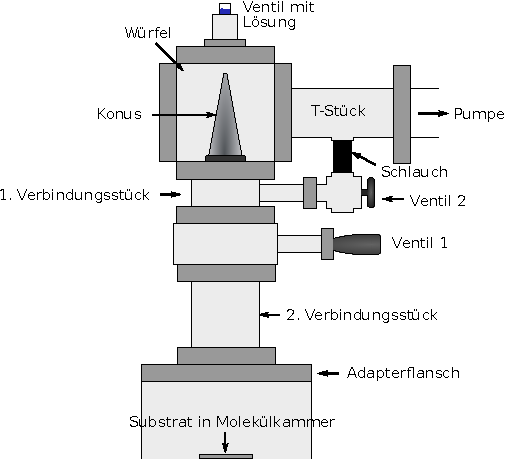
\includegraphics{bilder/wuerfelklein.pdf}
\end{figure}
\end{frame}


\begin{frame}
\frametitle{Aufbau der Apparatur}
\begin{figure}[H]
\centering
%\sffamily
\includesvg[svgpath=bilder/]{sb}
\end{figure}
\end{frame}

%___________________________________________________________________________________________________________________________________________
%___________________________________________________________________________________________________________________________________________


\subsection[Ergebnisse]{Test der Apparatur}

\begin{frame}
\frametitle{}
%\framesubtitle{Subtitles are optional}
\begin{itemize}
  \item
  \item
\end{itemize}
\end{frame}


%___________________________________________________________________________________________________________________________________________
%___________________________________________________________________________________________________________________________________________
%___________________________________________________________________________________________________________________________________________



\section*{Summary}

\begin{frame}
\frametitle<presentation>{Summary}

\begin{itemize}
  \item The \alert{first main message} of your talk in one or two lines.
\end{itemize}




% The following outlook is optional.
\vskip0pt plus.5fill
\begin{itemize}
  \item Outlook
  \begin{itemize}
    \item Something you haven't solved.
    \item Something else you haven't solved.
  \end{itemize}
\end{itemize}
\end{frame}

\end{document}
